\begin{figure}[t]
\begin{center}
% \psfig{figure=fft-block.eps,width=3in}
% \caption{The multi-stage FFT algorithm.
% \protect\label{fig:fftfilter}}
% \vspace{12pt}
%
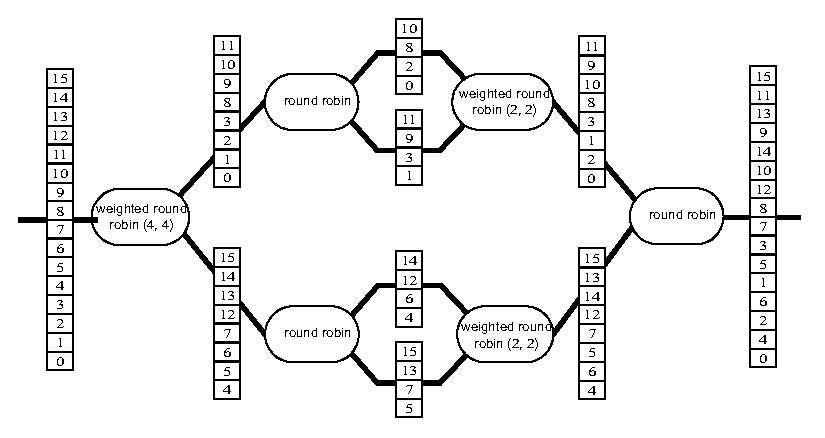
\includegraphics[width=3.53in]{fft-pre-tape.eps}
%\psfig{figure=fft-pre-tape.eps,width=3.53in}
\vspace{-6pt}
\caption{The bit-reversal phase in the FFT, with N=8.  A bit-reversal permutation is one that swaps all elements with indices whose binary representations are the reverse of each other.  The Butterfly stage is similar, but ommitted for lack of space.
\protect\label{fig:bitreverseorder}}
\vspace{-18pt}
% \psfig{figure=fft-butterfly-tape.eps,width=4.75in}
% \vspace{-6pt}
% \caption{The 4x4 butterfly stage in the FFT.
% \protect\label{fig:butterfly}}
\end{center}
\end{figure}

% \begin{figure}[t]
% \begin{minipage}{2.2in}
% \psfig{figure=fft-streamit.eps,width=162.35pt}
% \end{minipage}
% \hspace{0.2in}
% \begin{minipage}{2.4in}
% \centering
% \psfig{figure=fft-butterfly.eps,width=183.52pt}
% \end{minipage}
% \vspace{-12pt}
% \caption{The FFT stage of the software radio.  The Subtractor filter can be implemented in the same way as the Adder shown above, but is ommitted due to space considerations.
% \protect\label{fig:fft-streamit}}
% \end{figure}

% \begin{figure}
% \vspace{-0.4in}
% \begin{minipage}{2.5in}
% \psfig{figure=appendix-left.eps,width=180pt}
% \end{minipage}
% \begin{minipage}{2.5in}
% \psfig{figure=appendix-right.eps,width=197.64pt}
% \end{minipage}

% \begin{figure}
% \vspace{-0.4in}
% \tiny
% \begin{minipage}{2.5in}
% \begin{verbatim}
% class RFtoIF extends Filter {
%   int size, count;
%   float weight[];
%   void init(float f) {
%     input = new FloatChannel();
%     output = new FloatChannel();
%     setf(f);
%   }
%   void work() {
%     output.push(input.pop()*weight[count++]);
%     if (count==size) count = 0;
%   }
%   void setf(float f) {
%     count = 0;
%     size = CARRIER\_FREQ/f*N;
%     weight = new float[size];
%     for (int i=0; i<size; i++)
%       weight[i] = Math.sin(i*PI/size);
%   }
% }

% class Booster extends Pipeline {
%   void init(int N, boolean adds) {
%     if (adds) add(new FIR(N));
%   }
% }

% class CheckQuality extends Filter {
%   float aveHi, aveLo;
%   BoosterPortal booster;
%   boolean boosterOn;
%   void init(BoosterPortal booster, boolean on) {
%     input = new FloatChannel();
%     output = new FloatChannel();
%     aveHi = 0; aveLo = 1;
%     this.booster = booster;
%     this.boosterOn = on;
%   }
%   void work() {
%     float val = input.pop();
%     aveHi = max(0.9*aveHi, val);
%     aveLo = min(1.1*aveLo, val);
%     if (aveHi - aveLo < FAIL_QUAL && !booosterOn) {
%       booster.init(true, BEST_EFFORT);
%       boosterOn = true;
%     }
%     if (aveHi - aveLo > PASS_QUAL && boosterOn) {
%       booster.init(false, BEST_EFFORT);
%       boosterOn = false;
%     }
%     output.push(val);
%   }
% }

% class TrunkedRadio extends Pipeline {
%   int N = 64;
%   RFtoIFPortal freqHop = new RFtoIFPortal();
%   BoosterPortal onOff = new BoosterPortal().
%   void init() {
%     ReadFromAtoD in = add(new ReadFromAtoD());
%     RFtoIF rf2if = add(new RFtoIF(STARTFREQ));
%     Booster iss = add(new Booster(N, false));
%     add(new FFT(N));
%     add(new CheckFreqHop(freqHop));
%     add(new CheckQuality(onOff, false));
%     AudioBackEnd out = add(new AudioBackEnd());

%     freqHop.register(rf2if);
%     onOff.register(iss);
%     MAX_LATENCY(in, out, 10);
%   }
% }
% \end{verbatim}
% \end{minipage}
% \begin{minipage}{2in}
% \begin{verbatim}
% class CheckFreqHop extends SplitJoin {
%   RFtoIFPortal freqHop;
%   void init(RFtoIFPortal freqHop) {
%     this.freqHop = freqHop;
%     setSplitter(ROUND_ROBIN(N/4-2,1,1,N/2,1,1,N/4-2));
%     int k = 0;
%     for (int i=1; i<=5; i++) {
%       if ((i==2)||(i==4)) {
%         for (int j=0; j<2; j++) {
%           add(new Filter() {
%             void init() {
%               input = new FloatChannel();
%               output = new FloatChannel();
%             }
%             void work() {
%               float val = input.pop();
%               if (val >= MIN_THRESHOLD) 
%                 freqHop.setf(FREQ[k], new TimeInterval(4*N, 6*N)); 
%               output.push(val);
%             }});
%           k++;
%         }
%       } else add(new Identity());
%     }
%     setJoiner(ROUND_ROBIN(N/4-2,1,1,N/2,1,1,N/4-2));
%   }
% }

% class Butterfly extends Pipeline {
%   void init(int N, int W) {
%     add(new SplitJoin() {
%       void init() {
%         setSplitter(ROUND_ROBIN(N, N));
%         add(new Filter() {
%           float weight[] = new float[W];
%           int curr;
%           void init() {
%             input = new FloatChannel();
%             output = new FloatChannel();
%             for (int i=0; i<W; i++)
%               weight[i] = calcWeight(i, N, W);
%             curr = 0;
%           }
%           void work() {
%             output.push(input.pop()*weight[curr++]);
%             if(curr>= W) curr = 0;
%           }});
%         add(new Identity());
%         setJoiner(ROUND_ROBIN());
%     }});
%     add(new SplitJoin() {
%       void init() {
%         setSplitter(DUPLICATE());
%         add(new Filter() {
%           void init() {
%             input = new FloatChannel();
%             output = new FloatChannel();
%           }
%           void work() {
%             output.push(input.pop() - input.pop());
%           }});
%         add(new Filter() {  
%           void init() {
%             input = new FloatChannel();
%             output = new FloatChannel();
%           }
%           void work() {
%             output.push(input.pop() + input.pop());
%           }});
%         setJoiner(ROUND_ROBIN(N, N));
%     }});
% }
% \end{verbatim}
% \end{minipage}

% \vspace{-6pt}
% \caption{\protect\small A Trunked Radio Receiver in StreamIt.  The radio makes use of the FIR Filter and FFT that are defined in Figures~\ref{fig:firstreamit} and~\ref{fig:fft}, respectively.
% \protect\label{fig:radiocode}}
% \vspace{-12pt}
% \end{figure}







